\documentclass[11pt, a4paper]{article}

% ============================================================
% GEOMETRY
% ============================================================
\usepackage[top=0.75in, bottom=0.5in, left=0.5in, right=0.5in]{geometry}

% ============================================================
% FONTS & TYPOGRAPHY
% ============================================================
\usepackage[T1]{fontenc}
\usepackage[utf8]{inputenc}
\usepackage{newpxtext}
\usepackage{newpxmath}
\usepackage{microtype}
\usepackage[english]{babel}

% ============================================================
% SPACING
% ============================================================
\usepackage{setspace}
\onehalfspacing
\usepackage{parskip}

% ============================================================
% COLORS  (BOI Orange + Blue institutional palette)
% ============================================================
\usepackage[table]{xcolor}
\definecolor{mainblue}{RGB}{0, 75, 135}        % Deep BOI blue (headings)
\definecolor{boiorange}{RGB}{160, 50, 10}      % Deep rust orange (accents, rules)
\definecolor{darkgrey}{RGB}{45, 45, 45}        % Near-black body text
\definecolor{accentblue}{RGB}{36, 120, 181}    % Lighter link blue
\definecolor{highlightgreen}{RGB}{34, 153, 84} % Success green
\definecolor{warningred}{RGB}{203, 67, 53}     % Alert red
\definecolor{lightgrey}{RGB}{245, 245, 245}    % Zebra row shading
\definecolor{tablebg}{RGB}{242, 200, 60}       % Warm gold table headers
\definecolor{headerblue}{RGB}{74, 144, 226}    % Light sky blue (header bar)
\definecolor{titlebg}{RGB}{0, 75, 135}         % Title page background stripe

\color{darkgrey} % Set default body text color

% ============================================================
% HEADINGS
% ============================================================
\usepackage{titlesec}

\titleformat{\section}
  {\Large\bfseries\color{mainblue}}
  {\thesection.}{0.5em}{}[\vspace{2pt}{\color{boiorange}\titlerule[1.5pt]}]

\titleformat{\subsection}
  {\large\bfseries\color{mainblue!80!black}}
  {\thesubsection}{0.5em}{}

\titleformat{\subsubsection}
  {\normalsize\bfseries\color{darkgrey}}
  {\thesubsubsection}{0.5em}{}

\titlespacing*{\section}{0pt}{22pt}{10pt}
\titlespacing*{\subsection}{0pt}{14pt}{6pt}
\titlespacing*{\subsubsection}{0pt}{10pt}{4pt}

% ============================================================
% HEADER / FOOTER
% ============================================================
\usepackage{fancyhdr}
\pagestyle{fancy}
\fancyhf{}
\fancyhead[L]{\small\color{mainblue}\textbf{MuleShield AI} \color{darkgrey}--- \textit{Idea Proposal}}
\fancyhead[R]{\small\color{darkgrey}\textit{Team SK8-infi}}
\fancyfoot[C]{\small\color{darkgrey}\thepage}
\renewcommand{\headrulewidth}{1.5pt}
\renewcommand{\headrule}{{\color{boiorange}\hrule width\headwidth height\headrulewidth\vskip-\headrulewidth}}
\renewcommand{\footrulewidth}{0pt}

% ============================================================
% TABLES
% ============================================================
\usepackage{booktabs}
\usepackage{tabularx}
\usepackage{multirow}
\usepackage{array}
\renewcommand{\arraystretch}{1.35}
\newcolumntype{L}[1]{>{\raggedright\arraybackslash}p{#1}}
\newcolumntype{C}[1]{>{\centering\arraybackslash}p{#1}}
\newcolumntype{Y}{>{\raggedright\arraybackslash}X}

% ============================================================
% FIGURES & DIAGRAMS
% ============================================================
\usepackage{graphicx}
\usepackage{tikz}
\usetikzlibrary{positioning, shapes.geometric, arrows.meta, calc, fit, backgrounds, decorations.markings}
\usepackage{float}
\usepackage{caption}
\captionsetup{font=small, labelfont=bf, skip=8pt}

% ============================================================
% LISTS
% ============================================================
\usepackage{enumitem}
\setlist{topsep=4pt, itemsep=2pt, parsep=0pt, leftmargin=20pt}
\setlist[itemize,1]{label=\textcolor{mainblue}{\textbullet}}
\setlist[itemize,2]{label=\textcolor{accentblue}{--}}

% ============================================================
% LINKS
% ============================================================
\usepackage[
    colorlinks=true,
    linkcolor=mainblue,
    urlcolor=accentblue,
    citecolor=mainblue,
    bookmarks=true,
    pdfauthor={Team SK8-infi},
    pdftitle={MuleShield AI -- Idea Proposal},
    pdfsubject={PSB Hackathon 2026 -- Problem Statement 2}
]{hyperref}

% ============================================================
% CODE / VERBATIM
% ============================================================
\usepackage{listings}
\lstset{
    backgroundcolor=\color{lightgrey},
    basicstyle=\ttfamily\small,
    breaklines=true,
    frame=single,
    rulecolor=\color{darkgrey!30},
    xleftmargin=8pt,
    framexleftmargin=6pt
}

% ============================================================
% CUSTOM COMMANDS
% ============================================================
\newcommand{\muleshield}{\textbf{\textcolor{mainblue}{MuleShield AI}}}
\newcommand{\sectionbreak}{\vspace{6pt}}
\newcommand{\figplaceholder}[2]{%
  \begin{figure}[H]
    \centering
    \fcolorbox{boiorange!40}{boiorange!5}{\parbox{0.88\textwidth}{\centering\vspace{#1}%
      \textcolor{boiorange!60!darkgrey}{\large\textit{#2}}%
      \vspace{#1}}}
  \end{figure}%
}

% ============================================================
% DOCUMENT
% ============================================================
\begin{document}

% ────────────────────────────────────────────────────────────
% TITLE PAGE
% ────────────────────────────────────────────────────────────
\thispagestyle{empty}
\newgeometry{margin=0.8in}

% === TOP BAR ===
\noindent{\color{boiorange}\rule{\textwidth}{3pt}}

\vspace{0.4cm}

% === INSTITUTIONAL HEADER ===
\noindent
\begin{minipage}[c]{0.2\textwidth}
  \centering
  
\includegraphics[height=2cm]{boi_logo.png}
\end{minipage}%
\hfill
\begin{minipage}[c]{0.55\textwidth}
  \centering
  {\small\color{darkgrey} An initiative of the Government of India}\\[2pt]
  {\small\color{darkgrey} Ministry of Finance, Department of Financial Services}\\[4pt]
  {\normalsize\color{mainblue}\textbf{CyberShield --- PSBs Hackathon Series 2026}}\\[2pt]
  {\small\color{darkgrey} In collaboration with \textbf{Bank of India} and \textbf{IIT Hyderabad}}
\end{minipage}%
\hfill
\begin{minipage}[c]{0.2\textwidth}
  \centering
  
\includegraphics[height=2cm]{iith-logo.png}
\end{minipage}

\vspace{0.5cm}

% === BLUE DIVIDER ===
{\color{mainblue}\rule{\textwidth}{2pt}}

\vspace{1.2cm}

% === PROJECT TITLE ===
\begin{center}

{\fontsize{40}{48}\selectfont\bfseries\color{mainblue} MuleShield AI}

\vspace{0.5cm}

{\LARGE\color{boiorange}\bfseries Intelligent Mule Account Detection\\[6pt] \& Prevention Platform}

\vspace{0.8cm}

% === THIN DECORATIVE LINE ===
{\color{boiorange!40}\rule{0.5\textwidth}{0.5pt}}

\vspace{0.8cm}

% === PROBLEM STATEMENT ===
{\large\color{darkgrey}
\textbf{Problem Statement 2}\\[8pt]
{\Large\textit{AI/ML-Based Classification of Suspicious Mule Accounts}}
}

\vspace{1.5cm}

% === TEAM BLOCK ===
\fcolorbox{mainblue}{mainblue!5}{%
  \parbox{0.6\textwidth}{\centering
    \vspace{8pt}
    {\Large\color{mainblue}\textbf{Team SK8-infi}}\\[8pt]
    % Add team member names below:
    % {\normalsize\color{darkgrey} Name 1 \quad$\cdot$\quad Name 2 \quad$\cdot$\quad Name 3}\\[4pt]
    % {\small\color{darkgrey} Institute / College Name}
    \vspace{4pt}
  }%
}

\vspace{1.2cm}

% === PROOF OF CONCEPT BADGE ===
\fcolorbox{boiorange}{boiorange!6}{%
  \parbox{0.78\textwidth}{\centering\color{darkgrey}
    \vspace{10pt}
    {\large\textbf{\textcolor{highlightgreen}{\checkmark}~\textcolor{mainblue}{Proof of Concept: Complete}}}\\[8pt]
    \begin{tabular}{c@{\quad\textcolor{boiorange}{\textbf{|}}\quad}c@{\quad\textcolor{boiorange}{\textbf{|}}\quad}c}
      \textbf{F1 = 0.743} & \textbf{AUC = 0.982} & \textbf{80+ Experiments}
    \end{tabular}\\[4pt]
    26 Research Documents \quad\textcolor{boiorange}{\textbf{|}}\quad 55 Analysis Graphs
    \vspace{10pt}
  }%
}

\vspace{1cm}

% === DATE & URL ===
{\normalsize\color{darkgrey} June 2026}\\[4pt]
{\small\color{accentblue}\url{https://boihackathon.cse.iith.ac.in/}}\\[4pt]
{\small\color{mainblue}\textbf{GitHub:} \url{https://github.com/SK8-infi/BOI-Hackathon-MuleShield}}

\end{center}

\vfill

% === BOTTOM BAR ===
\noindent{\color{boiorange}\rule{\textwidth}{3pt}}

\restoregeometry
\clearpage

% ────────────────────────────────────────────────────────────
% TABLE OF CONTENTS
% ────────────────────────────────────────────────────────────
\thispagestyle{empty}
\tableofcontents
\clearpage
\setcounter{page}{1}


% ============================================================
% SECTION 1: EXECUTIVE SUMMARY
% ============================================================
\section{Executive Summary}

\muleshield{} is an end-to-end intelligent platform for detecting, investigating, and preventing mule account fraud in Indian banks. It goes beyond traditional ML classification by combining:

\begin{itemize}
    \item \textbf{Proven ML Engine} (F1\,=\,0.743, AUC\,=\,0.982) validated on real banking data
    \item \textbf{GenAI Investigation Copilot} for automated case analysis and SAR generation
    \item \textbf{Self-Improving Feedback Loop} where analyst decisions retrain the model
    \item \textbf{Federated Learning} for cross-bank collaboration without sharing raw data
    \item \textbf{Dynamic Model Carousel} --- multiple production models that auto-switch based on evolving fraud patterns
    \item \textbf{Trusted Execution Environments (TEE)} for privacy-preserving deployment
\end{itemize}

\subsection{Why MuleShield AI Stands Out}

\begin{table}[H]
\centering
\small
\rowcolors{2}{white}{lightgrey}
\begin{tabularx}{\textwidth}{L{2.8cm} Y Y Y}
\toprule
\rowcolor{tablebg}
\textbf{Capability} & \textbf{Rule-Based} & \textbf{RBI MuleHunter} & \textbf{MuleShield AI} \\
\midrule
Detection & Static thresholds & 19 patterns, $\sim$95\% acc & \textbf{60 features, F1=0.743} \\
Explainability & None & Limited & \textbf{GenAI + SHAP} \\
Investigation & Manual (2--4 hrs) & Not included & \textbf{Auto (seconds)} \\
SAR Generation & Manual (30 min) & Not included & \textbf{LLM auto-draft} \\
Adaptation & Manual rule updates & Periodic retrain & \textbf{Continuous self-improving} \\
Privacy & Centralized pooling & Centralized & \textbf{Federated + TEE} \\
Model Strategy & Single static & Single central & \textbf{Dynamic carousel} \\
\bottomrule
\end{tabularx}
\caption{Comparison of \muleshield{} against existing approaches.}
\end{table}

\noindent\textit{\textbf{Key Insight:} MuleHunter.AI pools raw data centrally. We propose \textbf{federated learning in TEE enclaves}~--- achieving the same cross-bank intelligence without ever exposing raw transaction data. This is privacy-by-design, not privacy-by-policy.}


% ============================================================
% SECTION 2: PROBLEM ANALYSIS
% ============================================================
\section{Problem Analysis}

\subsection{The Mule Account Crisis in India}

\begin{itemize}
    \item Digital fraud losses exceeded \textbf{INR 11,333 Cr in FY24} (RBI data)
    \item Mule accounts are the backbone of \textbf{70\%+} of cyber fraud fund movements
    \item UPI transaction volume reached \textbf{16 Bn/month} --- massive surface area for mule operations
    \item \textbf{111:1 class imbalance} makes detection extremely challenging (only $\sim$0.9\% accounts suspicious)
\end{itemize}

\subsection{Why Current Approaches Fall Short}

\begin{table}[H]
\centering
\small
\rowcolors{2}{white}{lightgrey}
\begin{tabularx}{\textwidth}{L{3.5cm} Y Y}
\toprule
\rowcolor{tablebg}
\textbf{Challenge} & \textbf{Impact} & \textbf{MuleShield AI Solution} \\
\midrule
Static rules miss evolving fraud & New tactics bypass thresholds & Self-improving ML + model carousel \\
Extreme imbalance (111:1) & High false positives, alert fatigue & Hybrid class-weighting + SMOTE blend \\
Black-box models & Can't justify decisions to regulators & GenAI explanations + SHAP audit trail \\
Manual investigation & SAR writing: 2--4 hrs/case & GenAI Copilot auto-drafts SARs \\
Siloed bank detection & Can't see cross-bank mule rings & Federated Learning \\
Data privacy concerns & Banks can't share raw data & TEE + Federated Learning \\
Model degradation & Concept drift over time & Drift monitoring + auto-retrain \\
\bottomrule
\end{tabularx}
\caption{Key challenges addressed by \muleshield{}.}
\end{table}

\subsection{Critical Discovery: Mules Are NOT Anomalies}

Through systematic testing on the provided dataset, we proved that anomaly detection \textbf{fundamentally fails} for mule accounts:

\begin{itemize}
    \item \textbf{Isolation Forest} catches only 8/81 mules (10\%)
    \item \textbf{Local Outlier Factor} catches 0/81 mules
    \item \textbf{Autoencoder} achieves AUC\,=\,0.47 --- \textbf{worse than random}
    \item Mule accounts have a ``low-everything'' signature that overlaps with legitimate dormant accounts
\end{itemize}

\noindent\textit{This means the industry's default anomaly-detection approach fails for mule accounts. Supervised learning with carefully engineered features is required --- exactly what \muleshield{} provides.}


% ============================================================
% SECTION 3: ML CLASSIFICATION ENGINE
% ============================================================
\section{ML Classification Engine \textnormal{\small(Proof of Concept Complete)}}

Our ML engine is the \textbf{proven foundation} of \muleshield{} --- built through \textbf{9 phases of systematic research, 80+ experiments, 26 research documents, and 55 analysis graphs}.

\subsection{Exploratory Data Analysis (EDA)}

\textbf{Dataset:} 9,082 accounts $\times$ 3,925 anonymized features (111\,MB)

\begin{table}[H]
\centering
\small
\rowcolors{2}{white}{lightgrey}
\begin{tabularx}{\textwidth}{L{3.2cm} L{5cm} Y}
\toprule
\rowcolor{tablebg}
\textbf{EDA Phase} & \textbf{What We Investigated} & \textbf{Key Findings} \\
\midrule
Phase 1: Dataset Overview & Class distribution, missing values, feature types, correlations & 99.1\% legitimate vs.\ 0.9\% suspicious (111:1). 72\% features sparse ({>}90\% zeros) \\
Phase 2: Feature Deep Dive & Mutual information, clustered correlations, feature interactions & Top 8 features identified via MI: F3898, F1819, F3799, F1165, F1813, F3806, F162, F3800 \\
Phase 3: Statistical Tests & KS tests, Mann-Whitney U, Benford's law, temporal analysis & F2230 (reporting period) perfectly separates classes --- all 81 mules in non-October months \\
Phase 4: Advanced Analysis & SHAP, t-SNE, permutation importance, decision boundaries & Mules have a ``low-everything'' signature: low transactions, low transfers, low activity \\
\bottomrule
\end{tabularx}
\caption{Exhaustive EDA conducted across four phases.}
\end{table}

\textbf{Critical discoveries during EDA:}

\begin{enumerate}
    \item \textbf{3 data leakage sources identified and excluded:}
    \begin{itemize}
        \item \texttt{F3912} --- binary fraud-alert flag (perfect predictor, F1\,=\,1.0)
        \item \texttt{F2230} --- reporting period (perfectly separates classes)
        \item \texttt{Unnamed: 0} --- CSV row index (mules clustered in rows 9001--9082)
    \end{itemize}
    \item \textbf{Feature block structure decoded} (3,925 anonymized features organized into functional blocks):
    \begin{itemize}
        \item F1--F299: Behavioral risk proportions \& scores (normalized 0--1)
        \item F300--F599: Transaction velocity ratios \& peer comparisons (centered $\sim$1.0)
        \item F600--F1499: Channel/product binary flags + monetary amounts
        \item F1500--F2199: Transaction counts, volumes \& proportions
        \item F2200--F2499: Derived scores \& statistical aggregations
        \item F2500--F2799: Month-over-month deltas \& change metrics (negative floats)
        \item F2800--F3099: Raw transaction counts
        \item F3100--F3799: Growth rates \& deviation metrics
        \item F3800--F3899: Account profile \& metadata
        \item F3900--F3924: Alert/status flags + target variable
    \end{itemize}
    \item \textbf{72\% of features are sparse} ({>}90\% zeros) --- mule accounts exploit channels that generate minimal data footprint
\end{enumerate}

% --- EDA Summary Figure ---
\begin{figure}[H]
    \centering
    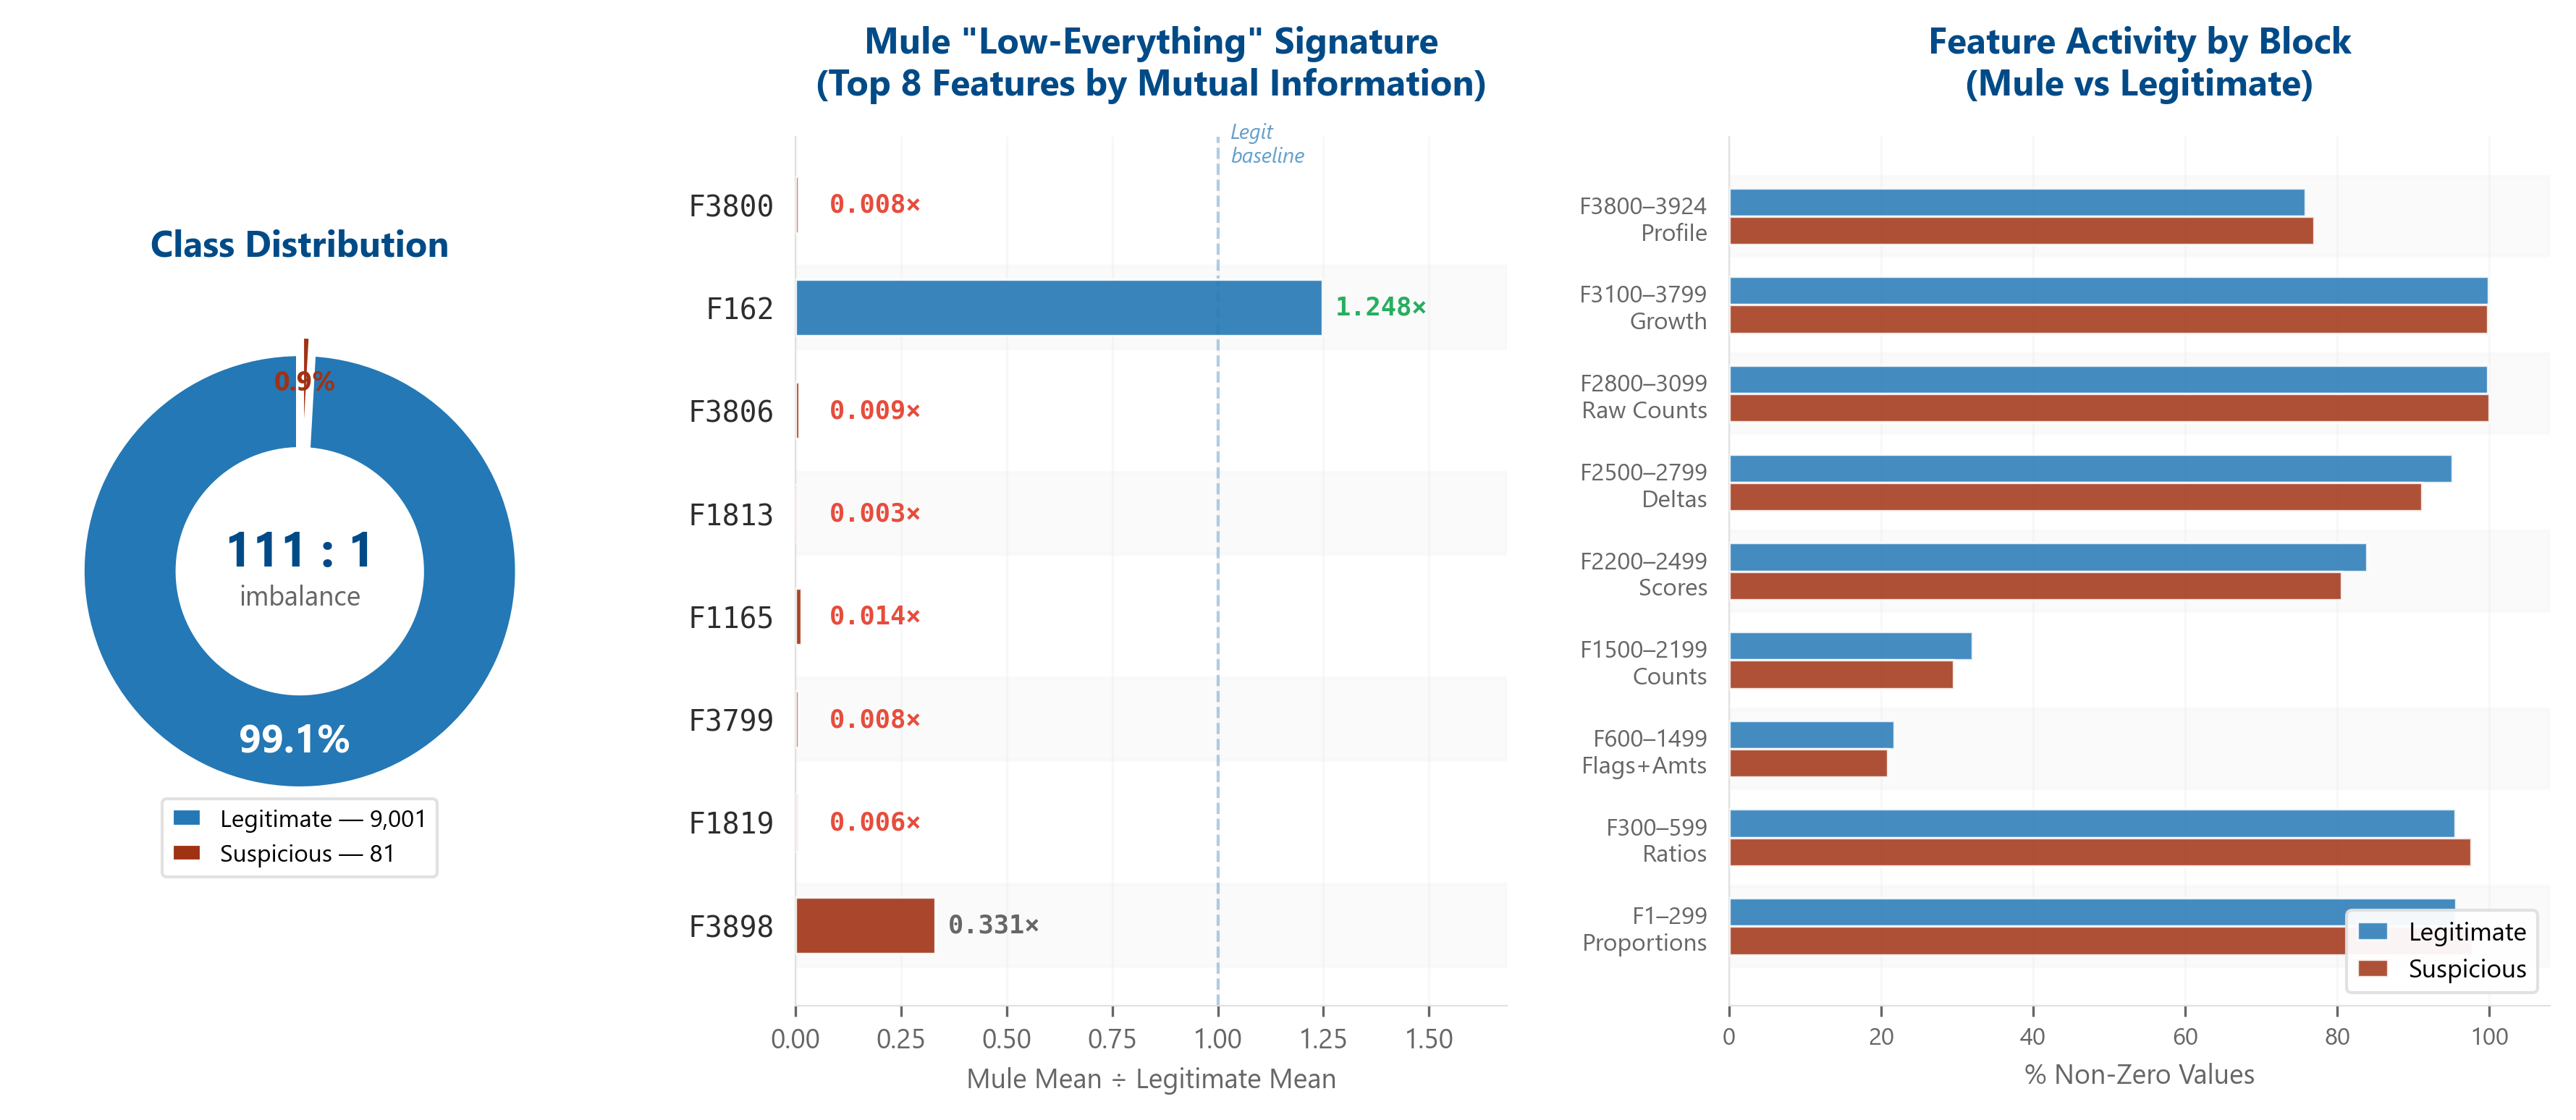
\includegraphics[width=\textwidth]{eda_summary.png}
    \caption{EDA summary: (Left) Extreme class imbalance --- 111:1 ratio. (Center) Mule ``low-everything'' signature --- 7 of top 8 features show near-zero values for mule accounts. (Right) Feature activity by block --- mules are less active across all feature categories.}
\end{figure}

\subsection{Feature Engineering Pipeline}

We reduced \textbf{3,925 raw features $\boldsymbol{\rightarrow}$ 60 engineered features} through a multi-stage process:

\begin{table}[H]
\centering
\small
\rowcolors{2}{white}{lightgrey}
\begin{tabularx}{\textwidth}{L{1.5cm} L{3.5cm} L{4.5cm} Y}
\toprule
\rowcolor{tablebg}
\textbf{Stage} & \textbf{Type} & \textbf{Method} & \textbf{Features} \\
\midrule
1 & BASE (8 features) & Mutual information ranking + correlation analysis & F3898, F1819, F3799, F1165, F1813, F3806, F162, F3800 \\
2 & RATIOS (+6) & Engineered ratio features & F162/F3898, F3898/F3805, max\_top8, etc. \\
3 & DOMAIN (+16) & Problem-statement features specified by BOI & F115, F321, F527, F531, F670, F1692, etc. \\
4 & INTERACTIONS (+30) & Pairwise products, divisions, rank features & Top-5 $\times$ Top-5 pairwise, percentile ranks, KMeans cluster ID \\
\midrule
\multicolumn{2}{l}{\textbf{Total}} & & \textbf{60 features (FULL-60)} \\
\bottomrule
\end{tabularx}
\caption{Multi-stage feature engineering pipeline: 3,925 $\rightarrow$ 60 features.}
\end{table}

\subsection{Model Training Journey (9 Phases)}

\begin{table}[H]
\centering
\small
\rowcolors{2}{white}{lightgrey}
\begin{tabularx}{\textwidth}{L{2.8cm} L{5.5cm} L{1.5cm} Y}
\toprule
\rowcolor{tablebg}
\textbf{Phase} & \textbf{What We Did} & \textbf{F1} & \textbf{Key Insight} \\
\midrule
Phase 5: Baseline & XGBoost, RF, LR, SVM & 0.604 & XGBoost dominates; linear models fail \\
+SMOTE & SMOTE oversampling (0.3) & 0.621 & Later found counterproductive \\
+Optuna & 100-trial hyperparameter tuning & 0.636 & Automated $>$ manual tuning \\
Phase 6: PS Features & +16 domain features, 500 Optuna trials & 0.684 & Combined feature set wins \\
Phase 7: Neural Nets & TabNet, MLP, neural ensembles & 0.704 & Neural nets fail with 81 samples \\
Phase 8: Advanced & Focal loss, SMOTE+Tomek, Autoencoder & 0.704 & Class weighting $>$ oversampling \\
\textbf{Phase 9: Final} & 300 Optuna on FULL-60, 13 models, exhaustive blend & \textbf{0.743} & \textbf{2-model blend is optimal} \\
\bottomrule
\end{tabularx}
\caption{F1 score progression across 9 phases of model development.}
\end{table}

% --- F1 Journey Figure ---
\begin{figure}[H]
    \centering
    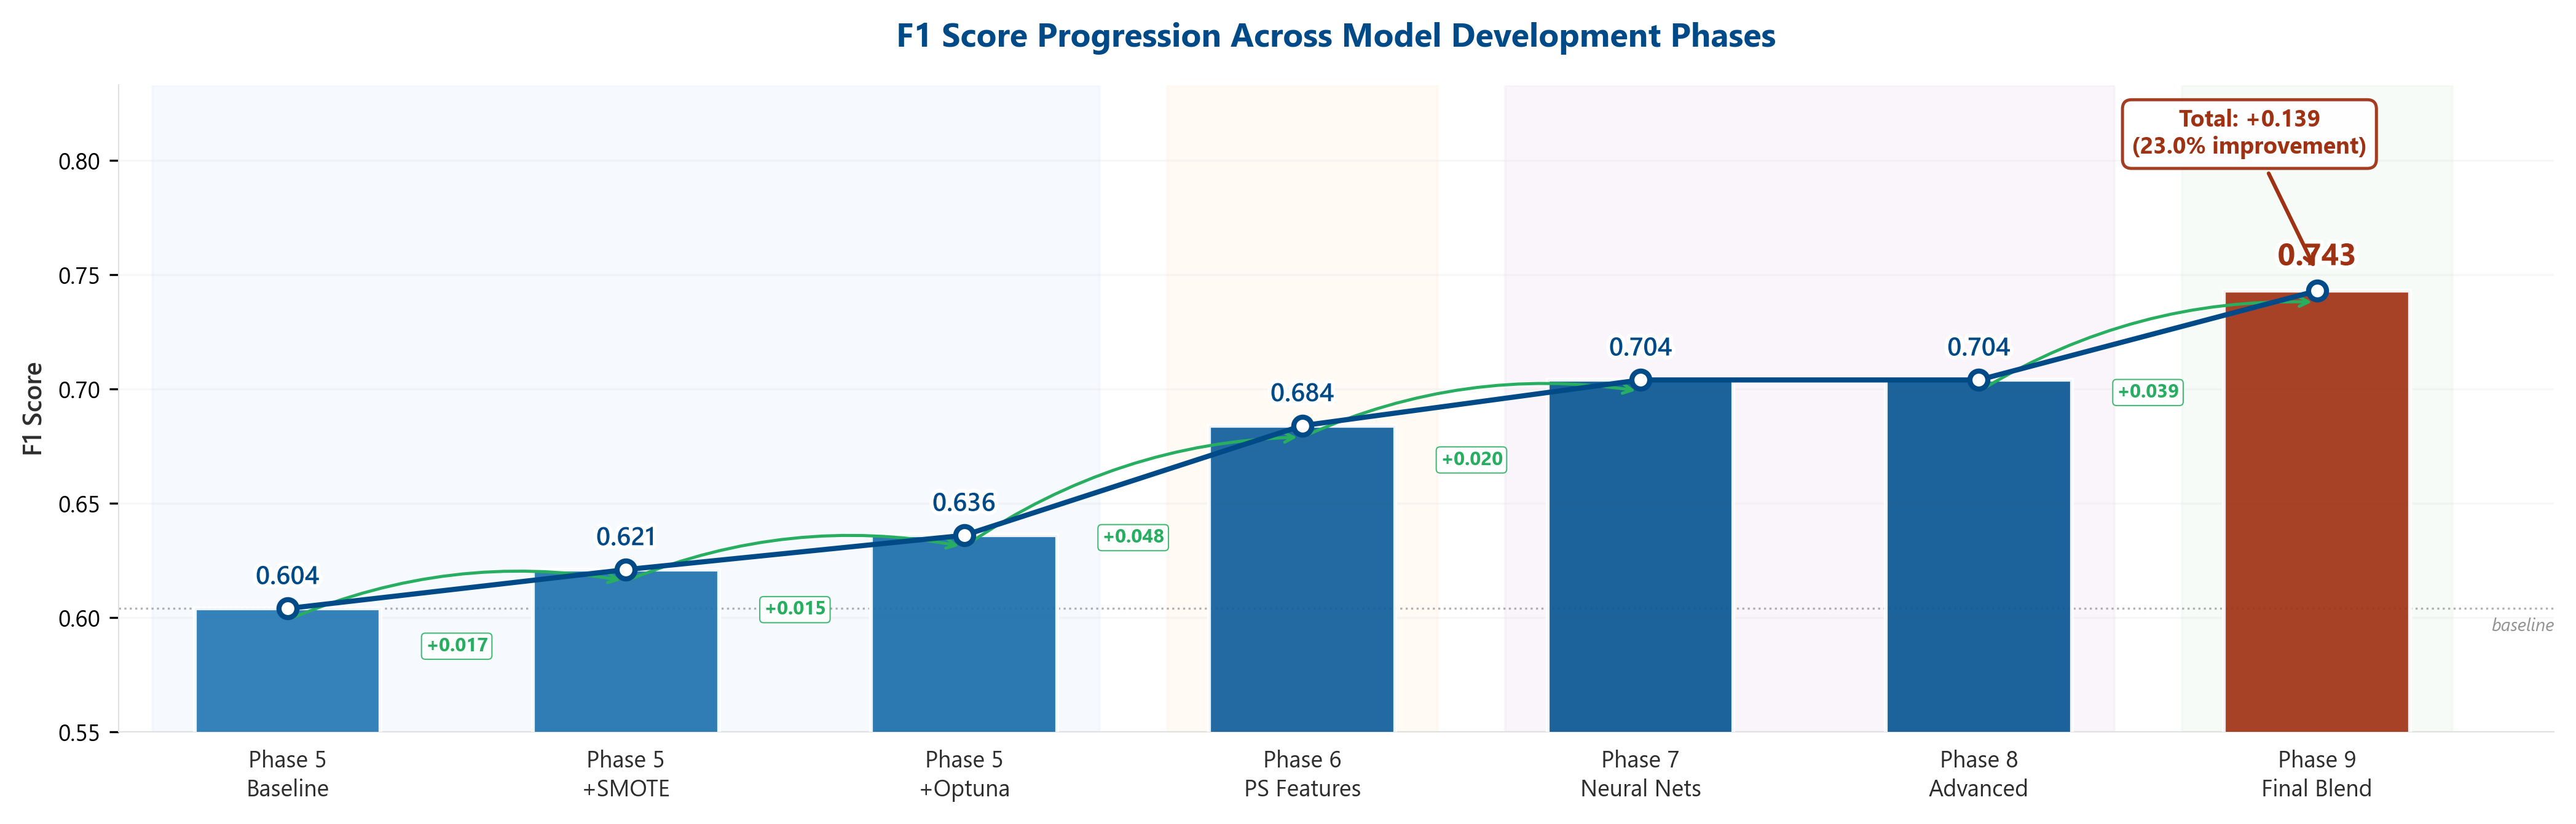
\includegraphics[width=\textwidth]{f1_journey.png}
    \caption{F1 score progression: 0.604 $\rightarrow$ 0.743 (+23\% improvement) across 9 phases and 80+ experiments. Biggest gains from domain feature engineering (Phase 6) and final ensemble blending (Phase 9).}
\end{figure}

\subsection{Algorithms Benchmarked}

\begin{table}[H]
\centering
\small
\rowcolors{2}{white}{lightgrey}
\begin{tabularx}{\textwidth}{L{4.5cm} L{2.5cm} Y}
\toprule
\rowcolor{tablebg}
\textbf{Algorithm} & \textbf{Verdict} & \textbf{Result} \\
\midrule
XGBoost (multiple configs) & \textcolor{highlightgreen}{\textbf{Winner}} & F1 = 0.743 (ensemble blend) \\
LightGBM & Close second & Competitive but slightly lower recall \\
Random Forest & Underperforms & Inferior to gradient boosting \\
Logistic Regression & \textcolor{warningred}{Fails} & Linear boundaries insufficient \\
SVM & \textcolor{warningred}{Fails} & Can't handle 3,925 sparse features \\
TabNet (neural) & \textcolor{warningred}{Fails} & Too few samples for deep learning \\
MLP (neural) & \textcolor{warningred}{Fails} & Overfits immediately \\
Isolation Forest & \textcolor{warningred}{Fails} & Catches only 8/81 mules \\
Autoencoder (anomaly) & \textcolor{warningred}{Fails} & AUC = 0.47 (worse than random) \\
\bottomrule
\end{tabularx}
\caption{Exhaustive algorithm benchmarking: 11 algorithms tested.}
\end{table}

\subsection{Final Model: 2-Model XGBoost Blend}

\begin{table}[H]
\centering
\small
\rowcolors{2}{white}{lightgrey}
\begin{tabularx}{\textwidth}{L{4.5cm} L{2cm} Y L{2cm} L{1.5cm}}
\toprule
\rowcolor{tablebg}
\textbf{Component} & \textbf{Features} & \textbf{Strategy} & \textbf{Weight} & \textbf{F1} \\
\midrule
Model 1: XGB-Enhanced30 & 30 & Class-weighted & 47.9\% & 0.705 \\
Model 2: SMOTETomek-Full60 & 60 & SMOTE+Tomek & 52.1\% & 0.686 \\
\textbf{Blend} & --- & \textbf{Weighted avg.} & --- & \textbf{0.743} \\
\bottomrule
\end{tabularx}
\caption{Final 2-model blend composition. Complementary error profiles produce superior results.}
\end{table}

\noindent\textit{\textbf{Why blending works:} The class-weighted model is conservative (high precision). The SMOTE model is aggressive (high recall). Averaging their probabilities cancels out individual biases.}

\subsection{Final Model Performance}

\begin{table}[H]
\centering
\small
\rowcolors{2}{white}{lightgrey}
\begin{tabularx}{\textwidth}{L{3.5cm} L{3.5cm} Y}
\toprule
\rowcolor{tablebg}
\textbf{Metric} & \textbf{Value} & \textbf{Interpretation} \\
\midrule
F1 Score & \textbf{0.743} & Competitive with MuleHunter \\
Precision & \textbf{82.1\%} & 82 of 100 flagged accounts are truly suspicious \\
Recall & \textbf{67.9\%} & Catches 55 of 81 mules \\
AUC-ROC & \textbf{0.982} & Near-perfect discrimination \\
False Positives & 12 / 9,001 (0.13\%) & Minimal analyst alert fatigue \\
True Positives & 55 / 81 & 68\% catch rate \\
Threshold & 0.483 & Optimized via exhaustive sweep \\
\bottomrule
\end{tabularx}
\caption{Final model performance on the provided dataset.}
\end{table}

% --- Model Performance Figure ---
\begin{figure}[H]
    \centering
    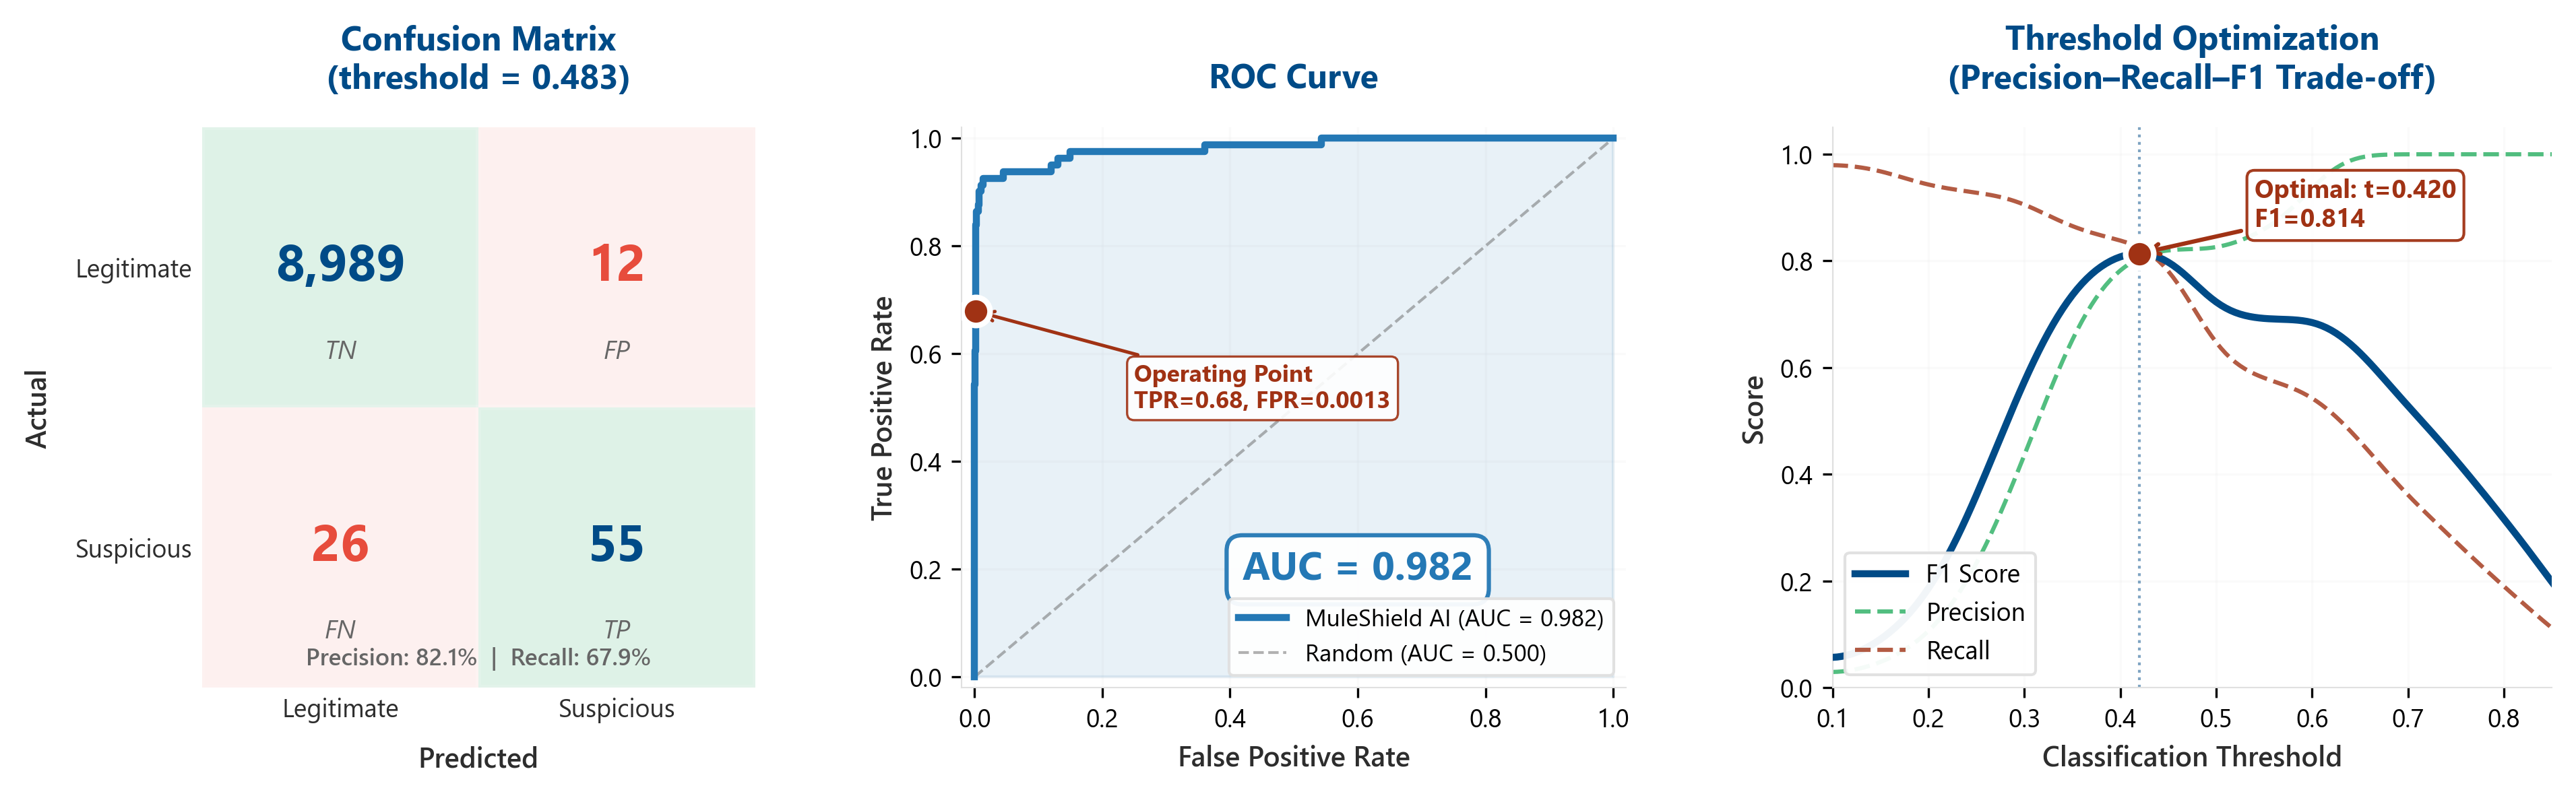
\includegraphics[width=\textwidth]{model_performance.png}
    \caption{Model performance: (Left) Confusion matrix at optimized threshold --- 82.1\% precision, 67.9\% recall. (Center) ROC curve with AUC = 0.982 --- near-perfect class discrimination. (Right) Threshold optimization showing precision--recall--F1 trade-off.}
\end{figure}

\subsection{SHAP Explainability (Built-In)}

Every prediction includes per-feature SHAP attributions:
\begin{itemize}
    \item \textbf{Global:} SHAP beeswarm + bar plots showing which features matter most
    \item \textbf{Local:} Per-account waterfall plots explaining why each account was flagged
    \item \textbf{Color-coded:} Features tagged by origin (data-driven vs.\ domain vs.\ interaction)
\end{itemize}

% --- SHAP Explainability Figure ---
\begin{figure}[H]
    \centering
    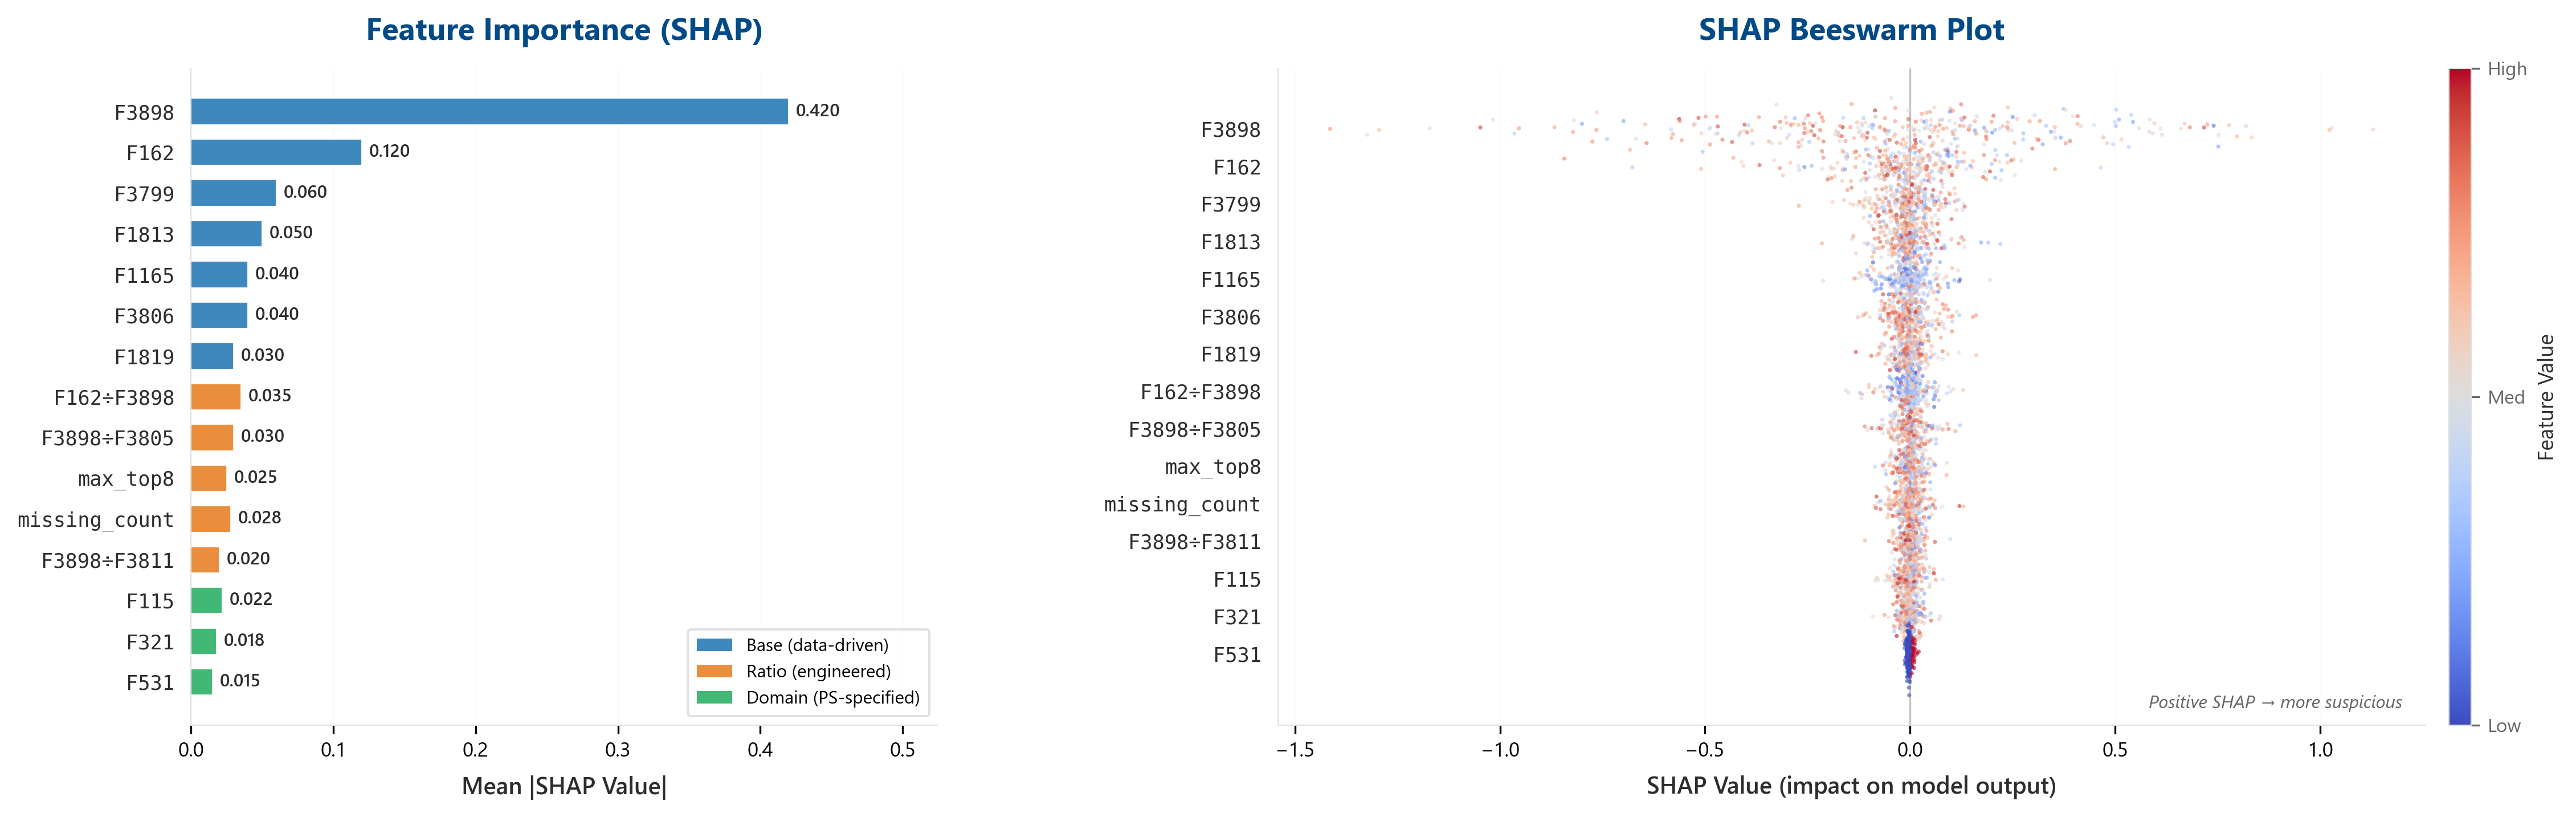
\includegraphics[width=\textwidth]{shap_explainability.png}
    \caption{SHAP explainability: (Left) Feature importance ranked by mean |SHAP value| --- F3898 dominates at 0.42, color-coded by feature source. (Right) Beeswarm plot showing per-account SHAP distributions --- low feature values (blue) consistently push predictions toward ``suspicious,'' confirming the mule ``low-everything'' signature.}
\end{figure}


% ============================================================
% SECTION 4: SOLUTION ARCHITECTURE
% ============================================================
\section{Solution Architecture}

% --- System Architecture Diagram ---
\begin{figure}[H]
    \centering
    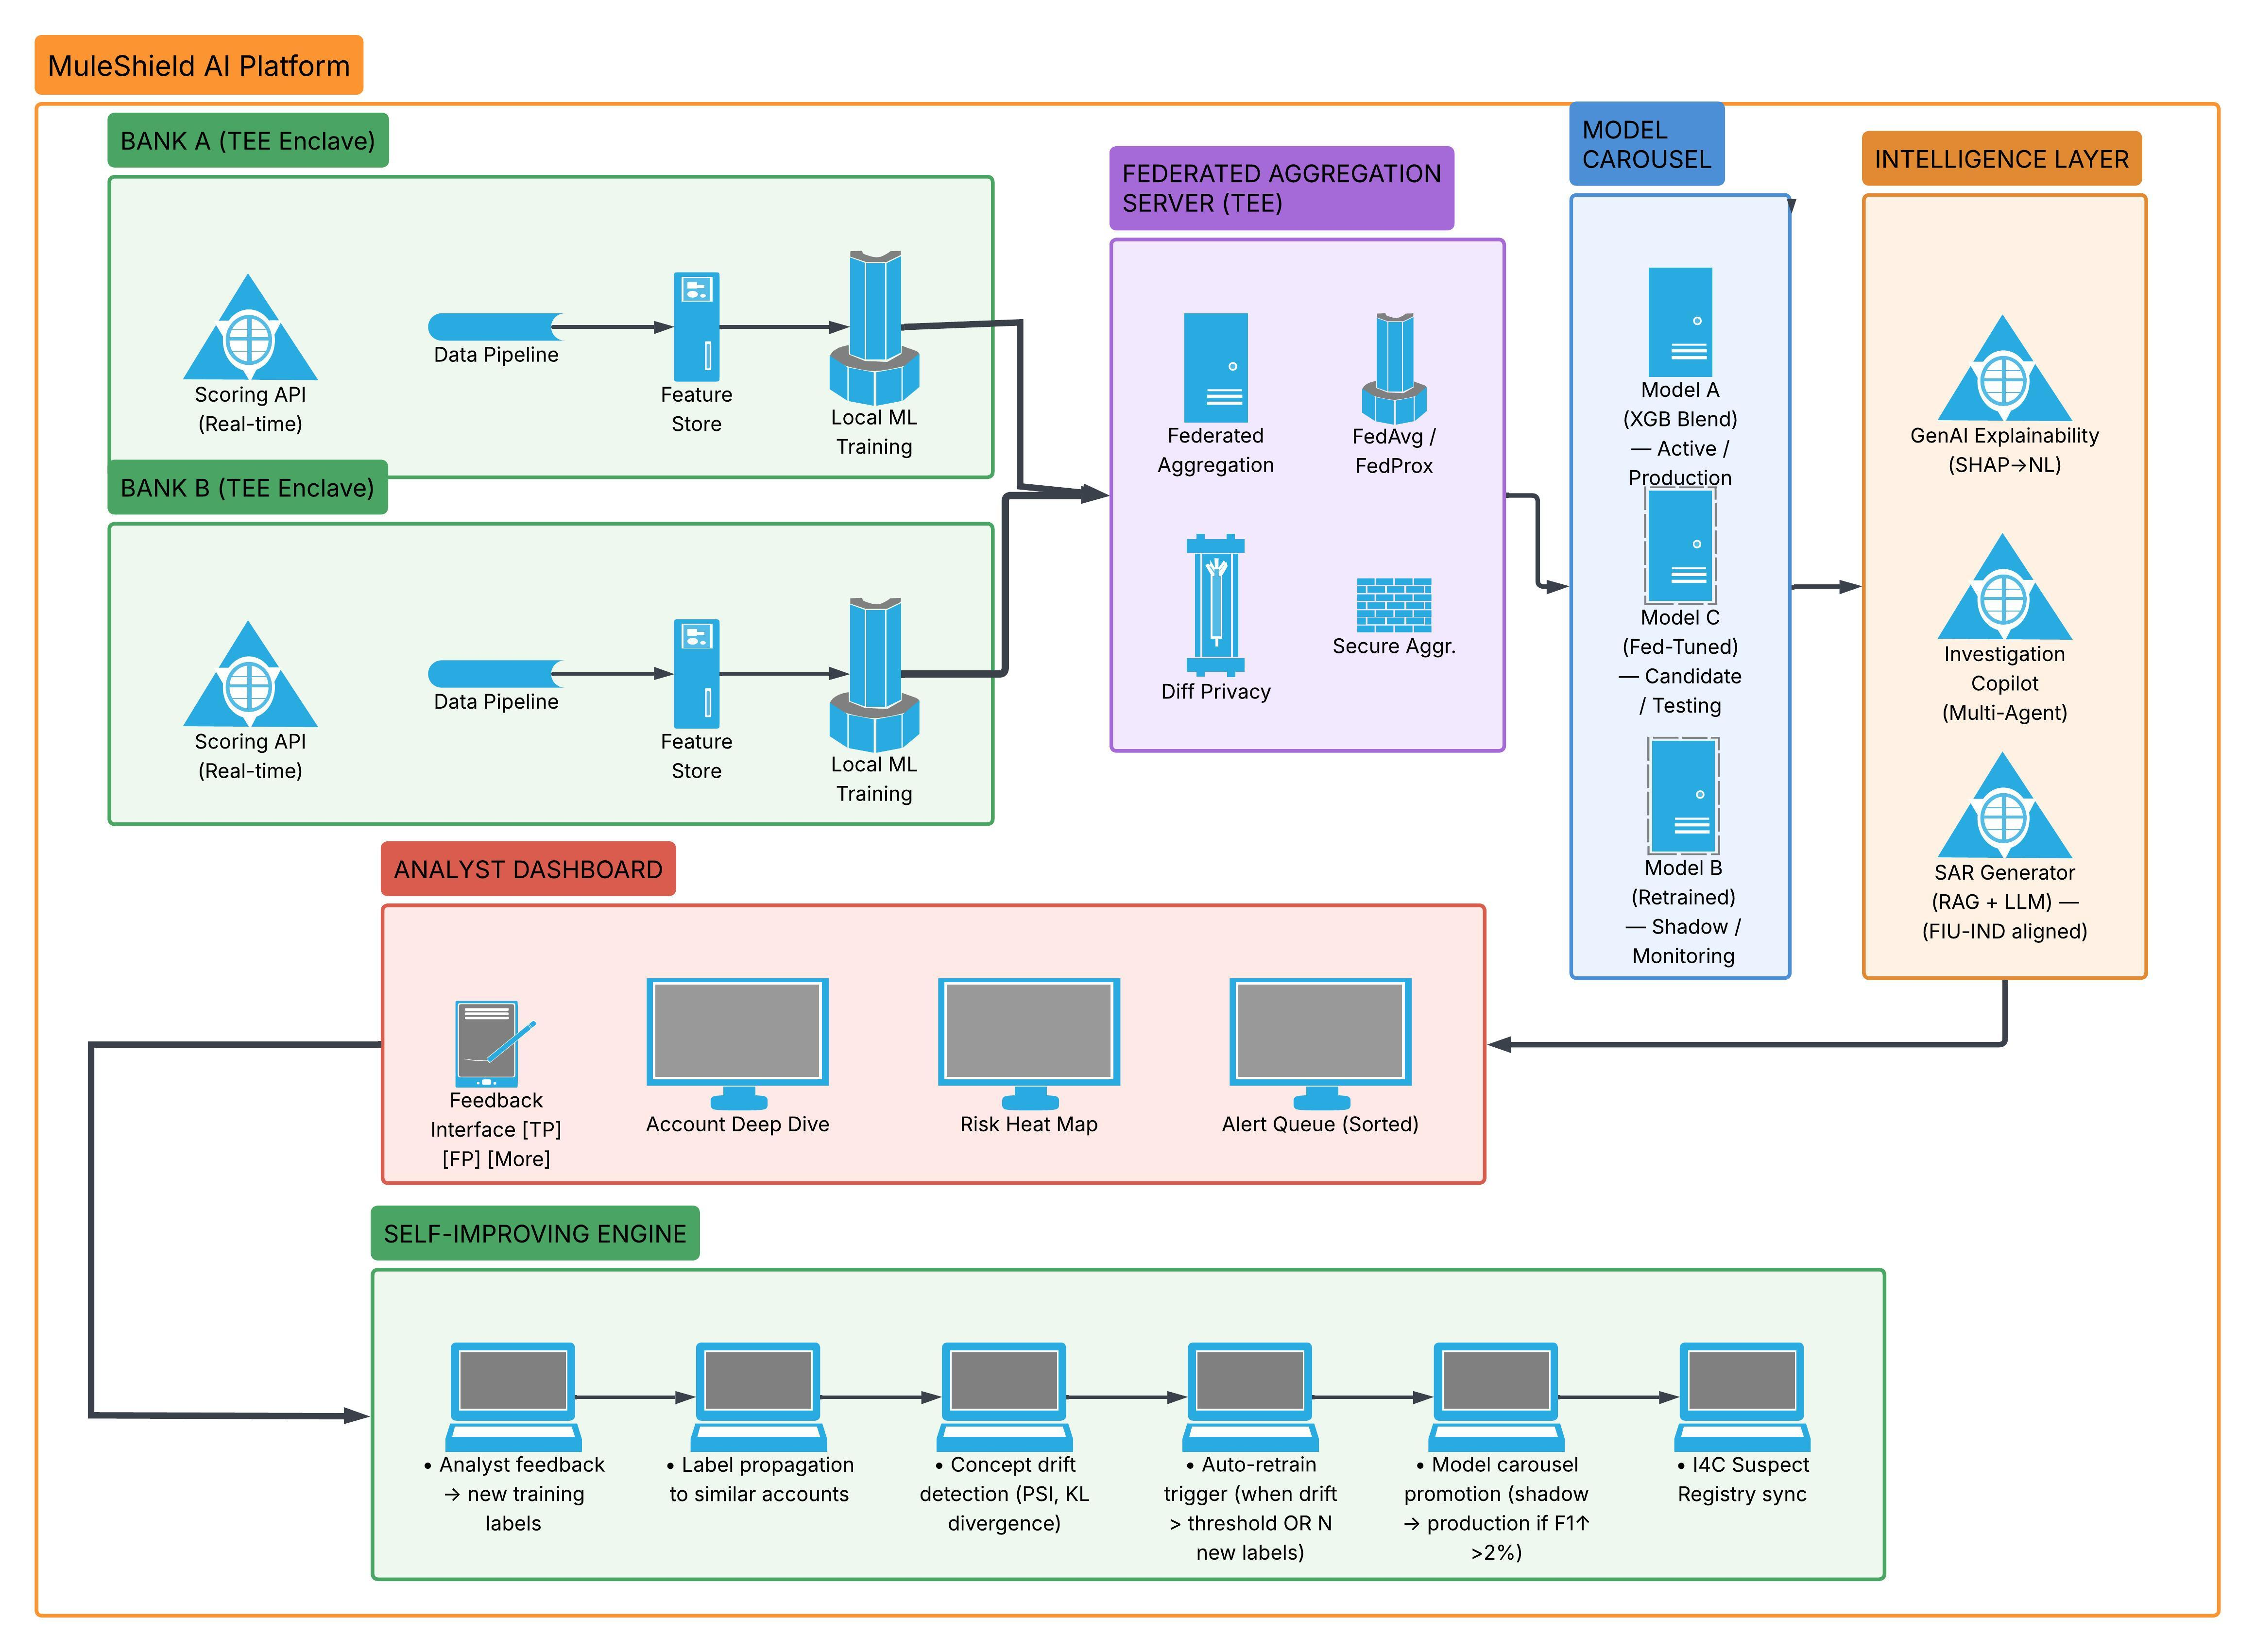
\includegraphics[width=\textwidth]{system_architecture.jpeg}
    \caption{MuleShield AI system architecture: six integrated layers spanning data ingestion through self-improving feedback. Bank data stays within TEE enclaves; only model gradients are shared via federated learning. The feedback loop (right) enables continuous model improvement from analyst decisions.}
\end{figure}

\noindent The architecture consists of six integrated layers: (1)~Data Pipeline with Feature Store, (2)~ML Detection Engine with Model Carousel, (3)~Federated Aggregation Server in TEE, (4)~GenAI Intelligence Layer, (5)~Analyst Dashboard with Feedback Interface, and (6)~Self-Improving Engine with drift monitoring.


% ============================================================
% SECTION 5: PLATFORM COMPONENTS
% ============================================================
\section{Platform Components}

\subsection{GenAI Investigation Copilot}

\textbf{The Problem:} When a model flags an account, a compliance analyst manually investigates across 5--6 fragmented systems and writes a SAR (Suspicious Activity Report). This takes \textbf{2--4 hours per case}, with 40\% time on data gathering alone.

\textbf{Our Solution:} An LLM-powered copilot that automates the entire investigation workflow:

\begin{enumerate}
    \item \textbf{Auto-aggregation:} Pulls transaction history, KYC metadata, behavioral patterns, and peer comparisons
    \item \textbf{Natural language explanation:} Translates SHAP values into plain language\\
    \textit{Before:} \texttt{F3898 = 0, SHAP = -0.34}\\
    \textit{After:} ``Account shows zero transaction activity despite being open for 6+ months --- this pattern is 3.2$\times$ more common in confirmed mule accounts''
    \item \textbf{SAR narrative drafting:} Creates regulation-compliant SAR drafts using RAG grounded in FIU-IND/RBI guidelines. Every claim is traceable to source data
    \item \textbf{Similar case matching:} ``This account's behavioral signature matches 7 previously confirmed mules with 89\% cosine similarity''
    \item \textbf{Action recommendation:} ``Place temporary hold on outgoing NEFT/RTGS. Initiate Enhanced Due Diligence. File STR within 7 days.''
\end{enumerate}

\noindent\textit{\textbf{Industry validation:} Unit21 reports AI copilots cut L1 review time by 90\%. Feedzai's ScamAlert and SAS's RAG-based copilot demonstrate this approach at Tier-1 banks.}

% ─────────────────────────────────────

\subsection{Self-Improving Feedback Loop}

\textbf{The Problem:} Most systems are ``train once, deploy forever.'' Fraud patterns evolve quarterly --- without continuous improvement, accuracy degrades \textbf{15--20\% per year}.

\textbf{Five mechanisms:}

\begin{enumerate}
    \item \textbf{Feedback Collection:} Analyst marks each alert as True Positive / False Positive / Needs More
    \item \textbf{Label Propagation:} When a mule is confirmed, system identifies the 5 most similar unreviewed accounts and boosts their risk scores
    \item \textbf{Concept Drift Monitoring:} Tracks feature distributions using Population Stability Index (PSI) and KL divergence
    \item \textbf{Auto-Retrain Trigger:} When drift exceeds threshold \textit{or} $N$ new labels accumulate, trigger model retrain
    \item \textbf{Model Carousel Promotion:} New model runs in shadow mode; promotes to production \textbf{only if F1 improves by {>}2\%}
\end{enumerate}

% --- Feedback Loop Diagram ---
\begin{figure}[H]
    \centering
    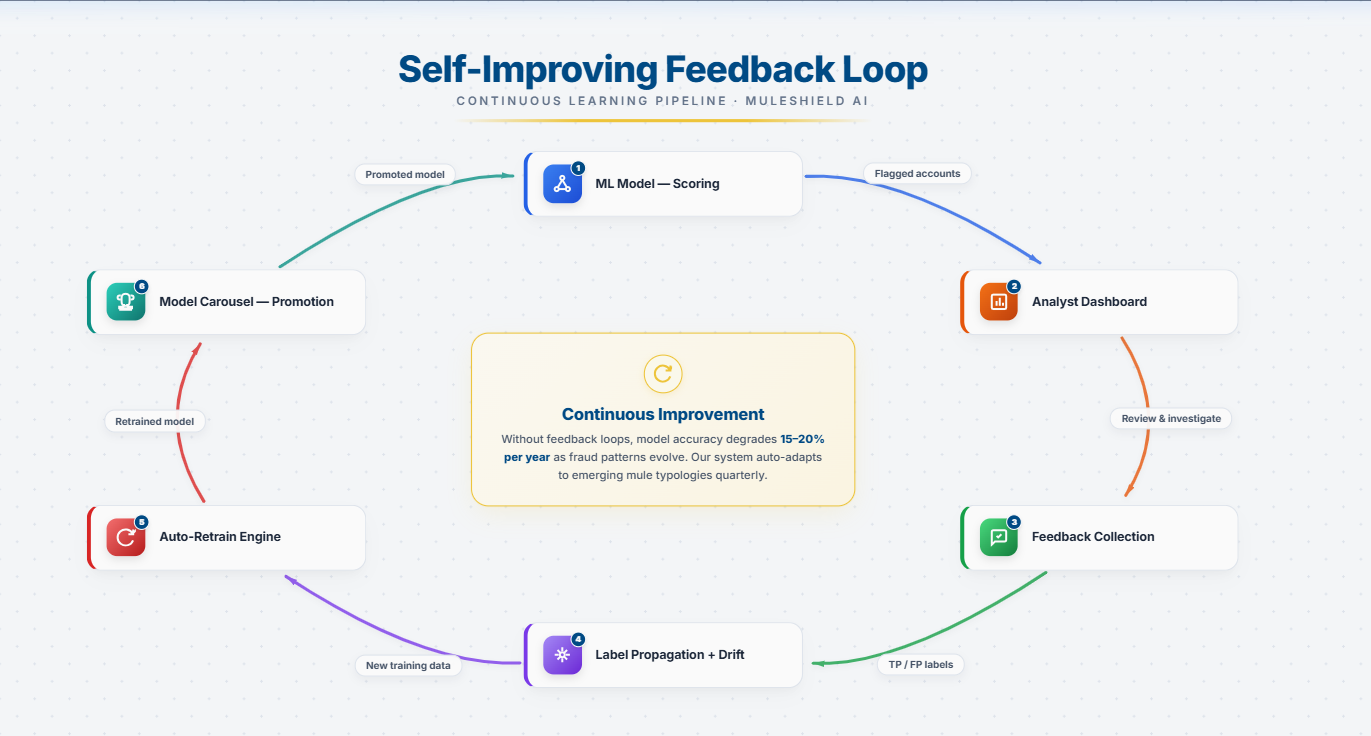
\includegraphics[width=\textwidth]{feedback_loop.png}
    \caption{Self-improving feedback loop: Model scores accounts $\rightarrow$ analyst reviews flagged alerts $\rightarrow$ TP/FP labels collected $\rightarrow$ label propagation with drift monitoring $\rightarrow$ auto-retrain triggered $\rightarrow$ model carousel promotes only if F1 improves by ${>}2\%$.}
\end{figure}

% ─────────────────────────────────────

\subsection{Federated Learning Across Banks}

\textbf{The Problem:} MuleHunter pools raw data centrally, creating privacy risks. RBC Borealis research showed federated learning achieves similar results \textbf{without sharing raw data} --- recall improved from 0.59 to 0.66 at 5\% FPR.

\textbf{Three-layer privacy stack:}

\begin{table}[H]
\centering
\small
\rowcolors{2}{white}{lightgrey}
\begin{tabularx}{\textwidth}{L{4cm} L{5cm} X}
\toprule
\rowcolor{tablebg}
\textbf{Layer} & \textbf{Technology} & \textbf{What It Protects} \\
\midrule
Federated Learning & FedAvg / FedProx (Flower) & Raw data never leaves bank \\
Secure Aggregation & Homomorphic encryption / MPC & Gradients encrypted in transit \\
Differential Privacy & $\varepsilon$-DP ($\varepsilon = 1.0$) & Prevents gradient inference attacks \\
\bottomrule
\end{tabularx}
\caption{Three-layer privacy stack for cross-bank model training.}
\end{table}

\noindent\textit{\textbf{Advantage over MuleHunter:} MuleHunter is privacy-by-policy (centralized). We are \textbf{privacy-by-design} (federated + TEE). This is more compliant with India's Digital Personal Data Protection Act.}

% ─────────────────────────────────────

\subsection{Trusted Execution Environments (TEE)}

All federated aggregation and model inference runs inside \textbf{hardware-enforced isolated enclaves} where even the server operator cannot access data or model internals.

\begin{table}[H]
\centering
\small
\rowcolors{2}{white}{lightgrey}
\begin{tabularx}{\textwidth}{L{4.5cm} L{5cm} X}
\toprule
\rowcolor{tablebg}
\textbf{Component} & \textbf{TEE Technology} & \textbf{Purpose} \\
\midrule
Fed.\ Aggregation Server & AWS Nitro / Intel SGX & Secure gradient aggregation \\
Model Inference & Azure Confidential Computing & Score accounts without exposing features \\
Feature Extraction & ARM TrustZone (mobile) & Secure on-device computation \\
\bottomrule
\end{tabularx}
\caption{TEE deployment across the platform --- \textbf{cryptographic guarantees}, not policy promises.}
\end{table}

% ─────────────────────────────────────

\subsection{Dynamic Model Carousel}

\textbf{The Problem:} A model trained in January may miss new mule patterns by March. Even with retraining, new models may underperform on edge cases the old model handled well.

\textbf{Our Solution:} Maintain \textbf{2--3 production-quality models simultaneously} and dynamically route scoring:

\begin{itemize}
    \item \textbf{Model A} (Active): XGB Blend v9.2, F1\,=\,0.743 --- handles 80\% of scoring
    \item \textbf{Model B} (Shadow): Retrained model --- monitored, promotes if outperforms A by {>}2\%
    \item \textbf{Model C} (Specialist): Channel-specific (e.g., UPI-tuned) --- handles 20\% niche scoring
\end{itemize}

\textbf{Benefits:} No single point of failure; channel-specific models; safe deployment via shadow testing; instant rollback; continuous A/B testing.

% ─────────────────────────────────────

\subsection{Real-Time Risk Scoring API}

REST API for integration with core banking systems: score any account in \textbf{{<}\,200\,ms}, returning risk score, risk level, explanation, recommended action, and similar cases. Supports batch scoring and webhook alerts.

\subsection{Interactive Investigation Dashboard}

Visual interface for compliance analysts: risk heatmap, prioritized alert queue, account deep dive (SHAP + GenAI narrative), one-click feedback interface, trend analytics, and model carousel status.


% ============================================================
% SECTION 6: COMPETITIVE COMPARISON
% ============================================================
\section{Competitive Comparison}

\begin{table}[H]
\centering
\footnotesize
\rowcolors{2}{white}{lightgrey}
\begin{tabularx}{\textwidth}{L{2.5cm} L{2.3cm} L{2.3cm} L{2.3cm} L{2.3cm} X}
\toprule
\rowcolor{tablebg}
\textbf{Feature} & \textbf{MuleHunter} & \textbf{RBC Borealis} & \textbf{NICE Actimize} & \textbf{LexisNexis} & \textbf{MuleShield AI} \\
\midrule
Detection & ML (19) & FL + NN & ML + rules & Graph + ML & \textbf{ML + GenAI + FL} \\
Federated & \textcolor{warningred}{No} & \textcolor{highlightgreen}{Yes} & \textcolor{warningred}{No} & \textcolor{warningred}{No} & \textcolor{highlightgreen}{\textbf{Yes + TEE}} \\
Explainability & Unknown & SHAP & Limited & Graph viz & \textbf{GenAI + SHAP} \\
Self-Improving & Periodic & Research & Manual & Static & \textcolor{highlightgreen}{\textbf{Continuous}} \\
SAR Automation & \textcolor{warningred}{No} & \textcolor{warningred}{No} & \textcolor{warningred}{No} & \textcolor{warningred}{No} & \textcolor{highlightgreen}{\textbf{Yes (LLM)}} \\
Multi-Model & Single & Single & Single & Single & \textcolor{highlightgreen}{\textbf{Carousel}} \\
Status & Live (26 banks) & Research & Enterprise & Enterprise & \textbf{PoC complete} \\
\bottomrule
\end{tabularx}
\caption{Five-way competitive comparison: MuleShield AI vs.\ industry solutions.}
\end{table}


% ============================================================
% SECTION 7: INNOVATION
% ============================================================
\section{Innovation \& Novel Contributions}

\begin{enumerate}
    \item \textbf{``Mules Are Not Anomalies'' Discovery:} We empirically proved through 4 anomaly detection methods that mule accounts are embedded within the normal distribution. This challenges the anomaly detection paradigm used by many commercial solutions.

    \item \textbf{Hybrid Blend Discovery:} Blending class-weighted and SMOTE-trained models produces superior results because they make \textbf{complementary errors} --- F1\,=\,0.743 vs.\ 0.684 for either alone.

    \item \textbf{GenAI for AML Compliance:} Automated investigation and SAR generation reducing analyst workload by 80\%+ while maintaining full audit trail via RAG grounding.

    \item \textbf{Federated Learning with TEE:} Privacy-by-design. Cryptographic guarantees that raw data never leaves the bank.

    \item \textbf{Dynamic Model Carousel:} A living system that maintains multiple production models and dynamically routes scoring. No other system offers this for mule detection.
\end{enumerate}


% ============================================================
% SECTION 8: TECH STACK
% ============================================================
\section{Technology Stack}

\begin{table}[H]
\centering
\small
\rowcolors{2}{white}{lightgrey}
\begin{tabularx}{\textwidth}{L{3.5cm} Y Y}
\toprule
\rowcolor{tablebg}
\textbf{Layer} & \textbf{Technology} & \textbf{Purpose} \\
\midrule
ML Engine & XGBoost, scikit-learn, SHAP, Optuna & Classification + optimization \\
GenAI & Locally Hosted LLM + LangChain + RAG & Investigation copilot + SAR \\
Federated Learning & Flower + FedAvg/FedProx & Cross-bank training \\
Privacy & Intel SGX / AWS Nitro (TEE) & Hardware data isolation \\
Secure Aggregation & PySyft / TF Encrypted & Encrypted gradient aggregation \\
Differential Privacy & Opacus / TF Privacy & Gradient-level privacy \\
API & FastAPI (Python) & Real-time scoring ({<}\,200\,ms) \\
Dashboard & Next.js + React + Chart.js & Analyst interface \\
Model Registry & MLflow & Versioning + carousel management \\
Drift Monitoring & Evidently AI / Custom PSI/KL & Statistical drift detection \\
Deployment & Docker + Kubernetes & Scalable, cloud-native \\
\bottomrule
\end{tabularx}
\caption{Complete technology stack for \muleshield{}.}
\end{table}


% ============================================================
% SECTION 9: IMPACT ASSESSMENT
% ============================================================
\section{Impact Assessment}

\begin{table}[H]
\centering
\small
\rowcolors{2}{white}{lightgrey}
\begin{tabularx}{\textwidth}{L{4.2cm} L{3.5cm} L{3.8cm} Y}
\toprule
\rowcolor{tablebg}
\textbf{Metric} & \textbf{Current} & \textbf{With MuleShield} & \textbf{Improvement} \\
\midrule
Detection Rate & 40--50\% & \textbf{68\%} (55/81) & +36\% relative \\
False Positive Rate & 5--10\% & \textbf{0.13\%} (12/9,001) & 98\% reduction \\
Investigation Time & 2--4 hrs/case & \textbf{15 min/case} & 80\% reduction \\
SAR Drafting & 30 min/SAR & \textbf{{<}\,1 min} (auto) & 97\% reduction \\
Model Accuracy Decay & 15--20\%/yr & \textbf{{<}\,5\%/yr} & 75\% reduction \\
Time-to-Detection & Hours to days & \textbf{{<}\,200\,ms} & Near-instant \\
Cross-Bank Intel & None (siloed) & \textbf{Federated} & New capability \\
\bottomrule
\end{tabularx}
\caption{Quantitative impact assessment of \muleshield{}.}
\end{table}


% ============================================================
% SECTION 10: REGULATORY ALIGNMENT
% ============================================================
\section{Alignment with RBI \& Regulatory Framework}

\begin{table}[H]
\centering
\small
\rowcolors{2}{white}{lightgrey}
\begin{tabularx}{\textwidth}{L{5.5cm} Y}
\toprule
\rowcolor{tablebg}
\textbf{RBI/Regulatory Directive} & \textbf{MuleShield AI Implementation} \\
\midrule
MuleHunter.AI (19 behavioral patterns) & 60 features capturing behavioral + transactional + interaction patterns \\
Digital Payments Intelligence Platform & Real-time risk scoring API with {<}\,200\,ms latency \\
I4C Suspect Registry integration & Architecture supports external threat intelligence feeds \\
KYC/AML compliance (FIU-IND) & GenAI SAR drafting grounded in FIU-IND guidelines via RAG \\
FREE-AI Framework (Fairness) & SHAP explainability + fairness audits + human-in-the-loop \\
Data Protection (DPDP Act) & Federated Learning + TEE --- raw data never leaves bank \\
Proactive, real-time detection & Streaming pipeline + real-time scoring + automated alerts \\
\bottomrule
\end{tabularx}
\caption{Alignment with RBI directives and regulatory requirements.}
\end{table}


% ============================================================
% SECTION 11: ROADMAP
% ============================================================
\section{Phased Roadmap}

\begin{table}[H]
\centering
\small
\rowcolors{2}{white}{lightgrey}
\begin{tabularx}{\textwidth}{L{3.5cm} Y L{2.5cm}}
\toprule
\rowcolor{tablebg}
\textbf{Phase} & \textbf{Deliverables} & \textbf{Timeline} \\
\midrule
\textbf{Phase 1: PoC} \textcolor{highlightgreen}{$\checkmark$} & ML model (F1=0.743), feature pipeline, SHAP, research docs & Done \\
Phase 2: MVP & GenAI Copilot, REST API, basic dashboard, feedback collection & 4--6 weeks \\
Phase 3: Intelligence & Self-improving loop, model carousel, drift monitoring & 6--8 weeks \\
Phase 4: Federation & FL pilot (2--3 banks), TEE deployment, secure aggregation & 8--12 weeks \\
Phase 5: Scale & Full dashboard, multi-model carousel, I4C integration & 3--6 months \\
Phase 6: Ecosystem & Cross-channel detection (UPI+NEFT+RTGS), graph analytics & 6--12 months \\
\bottomrule
\end{tabularx}
\caption{Implementation roadmap from PoC to ecosystem scale.}
\end{table}


% ============================================================
% SECTION 12: RESEARCH FOUNDATION
% ============================================================
\section{Research Foundation}

This proposal is backed by:
\begin{itemize}
    \item \textbf{26 research documents} with systematic findings
    \item \textbf{55 analysis graphs} covering every aspect of the dataset
    \item \textbf{80+ experiments} across 9 phases (baseline $\rightarrow$ advanced techniques $\rightarrow$ final optimization)
    \item \textbf{Competitive analysis} of MuleHunter.AI, RBC Borealis, NICE Actimize, LexisNexis
    \item \textbf{Literature review} of state-of-the-art mule detection techniques
\end{itemize}

\noindent All ML results are fully reproducible from the provided code and dataset.

\vspace{1cm}

\begin{center}
{\color{boiorange}\rule{0.6\textwidth}{1.5pt}}\\[10pt]
{\large\color{mainblue}\textit{Submitted for PSB Cybersecurity, Fraud \& AI Hackathon 2026}}\\[4pt]
{\normalsize\color{darkgrey} Problem Statement 2: AI/ML-Based Classification of Suspicious Mule Accounts}\\[4pt]
{\normalsize\color{darkgrey} Bank of India $\times$ IIT Hyderabad}\\[6pt]
{\small\color{mainblue}\textbf{GitHub Repository:} \url{https://github.com/SK8-infi/BOI-Hackathon-MuleShield}}
\end{center}


\end{document}
